%!TEX root = ../thesis.tex
%*******************************************************************************
%****************************** Fifth Chapter **********************************
%*******************************************************************************
\chapter{ER: Endoplasmic reticulum network dynamics} \label{chap:ER}

% Don't forget to PEE/L


% **************************** Define Graphics Path **************************
\ifpdf
    \graphicspath{{Chapter5/Figs/Raster/}{Chapter5/Figs/PDF/}{Chapter5/Figs/}}
\else
    \graphicspath{{Chapter5/Figs/Vector/}{Chapter5/Figs/}}
\fi

%``I have also just seen some of the data from Meng on lysosomes and ER tubules! I have never seen anything like this. This is only possible through your amazing efforts.''
%
%\textit{Gabi Kaminski, email 10-05-2018}

\section{Introduction}
\subsection{ER malfunction is linked to a variety of diseases}
The endoplasmic reticulum (ER) is an interconnected network of tubular pipes and reservoirs present in eukaryotic cells~\cite{alberts2002molecular}.
Its function includes the biogenesis of membrane and secretory proteins, and delivery of these functional solutes throughout the cell~\cite{dyson1978cell}.
Since the ER network extends to the cell periphery, molecules can be transported to distant sites in the cell.

When demand is greater than the capacity of ER to fold proteins, ER stress can occur~\cite{oakes2015role}.
ER stress can also be caused by proteins that cannot properly fold inside the ER~\cite{rao2004misfolded}.
A number of signal transduction proteins in the cell monitor proteins secreted by the ER, and if an imbalance is detected the ER stress response begins~\cite{oakes2015role}.

As the largest organelle in a cell, recent studies have shown ER forms membrane contacts with all other cellular organelles, with a higher number of contact sites than any other organelle-organelle interaction~\cite{phillips2016structure, valm2017applying}.
Since ER is found in almost all human cells, it is therefore not surprising that a wide range diseases have been associated with ER stress, including neurodegeneration, atherosclerosis, type 2 diabetes, liver disease, metabolic diseases, and cancer~\cite{oakes2015role, ozcan2012role}.

The rate at which luminal ER content is distributed affects the efficiency of ER-mediated intracellular connectivity~\cite{hubner2014membrane, blackstone2011hereditary}.
Understanding the fundamental processes of ER protein mobility is therefore vital to curing diseases caused by mutations in ER proteins.

\subsection{Flow in the ER is an active process}
ER proteins are delivered around the cell by moving through a network of tubes which make up the ER.
It has been shown with fluorescence recovery after photo-bleaching (FRAP) that protein mobility is an ATP-dependent process - that is, proteins move slower when ATP is depleted~\cite{dayel1999diffusion, nehls2000dynamics}.

More recently, we have shown with single particle tracking that molecules in the ER do not move with diffusive motion~\cite{holcman2018single}.
Rather, they have a fast, directed velocity as they flow along ER tubes, but move with slow, diffusive motion at nodes where 3 or more tubes connect, as shown in Figure~\ref{fig:er-directed-flow-velocity}.
Appendix~\ref{appn:flow} contains further details on the calculation of the flow models. 

\begin{figure}[b!]
\centering
	\begin{subfigure}[b]{0.4\textwidth}
		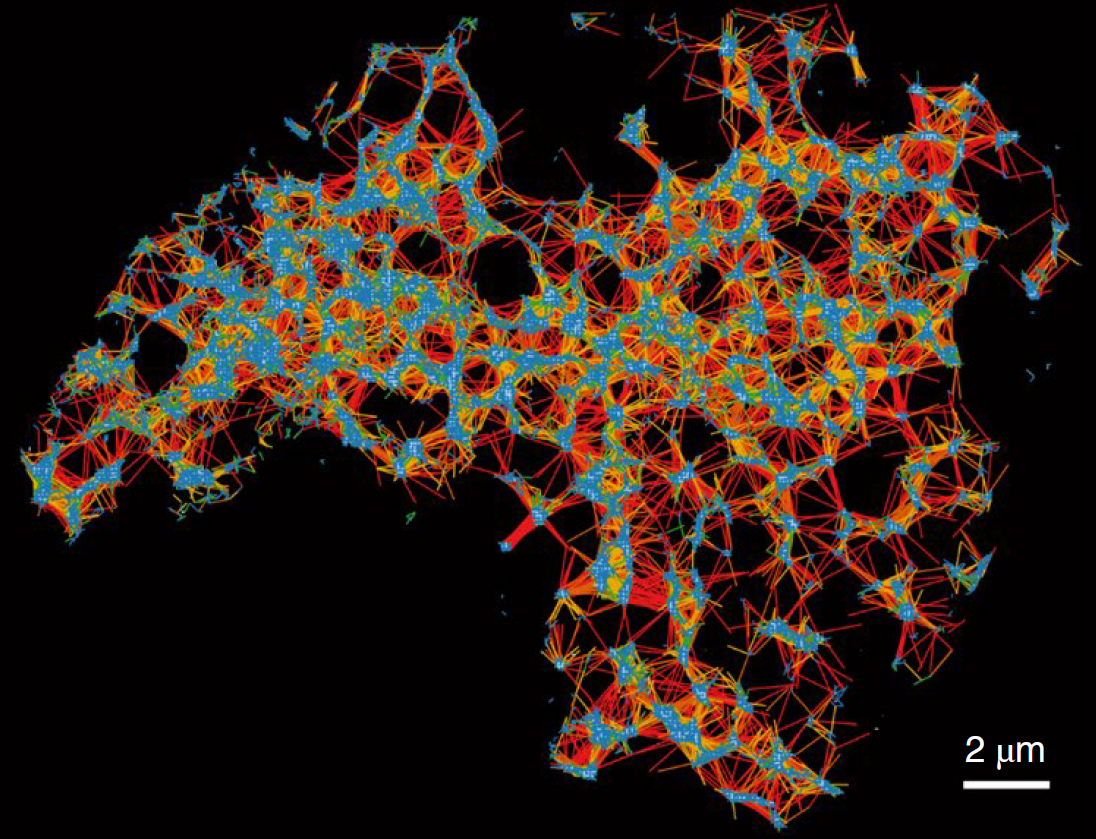
\includegraphics[width=1.0\textwidth]{er-directed-flow}
		\caption{} \label{fig:er-directed-flow-velocity}
	\end{subfigure}
	\hfill
	\begin{subfigure}[b]{0.29\textwidth}
		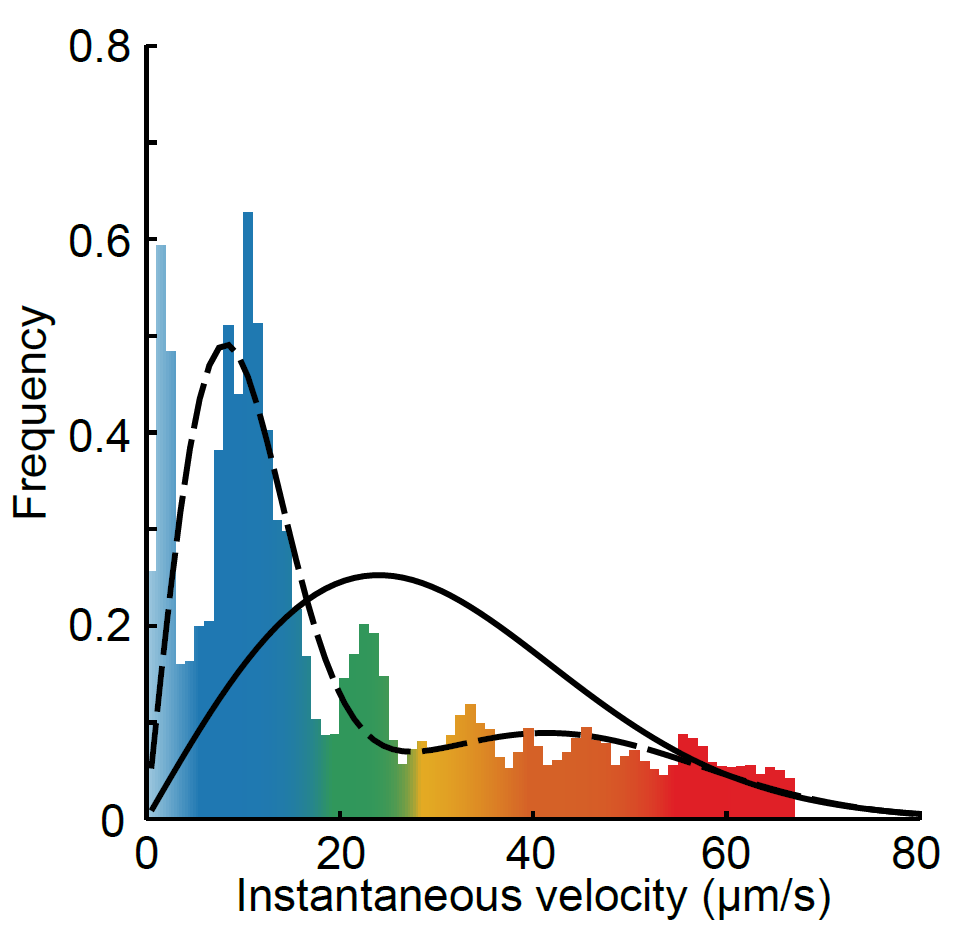
\includegraphics[width=1.0\textwidth]{er-directed-flow-distribution}
		\caption{} \label{fig:er-directed-flow-distribution}
	\end{subfigure}
	\hfill
	\begin{subfigure}[b]{0.29\textwidth}
		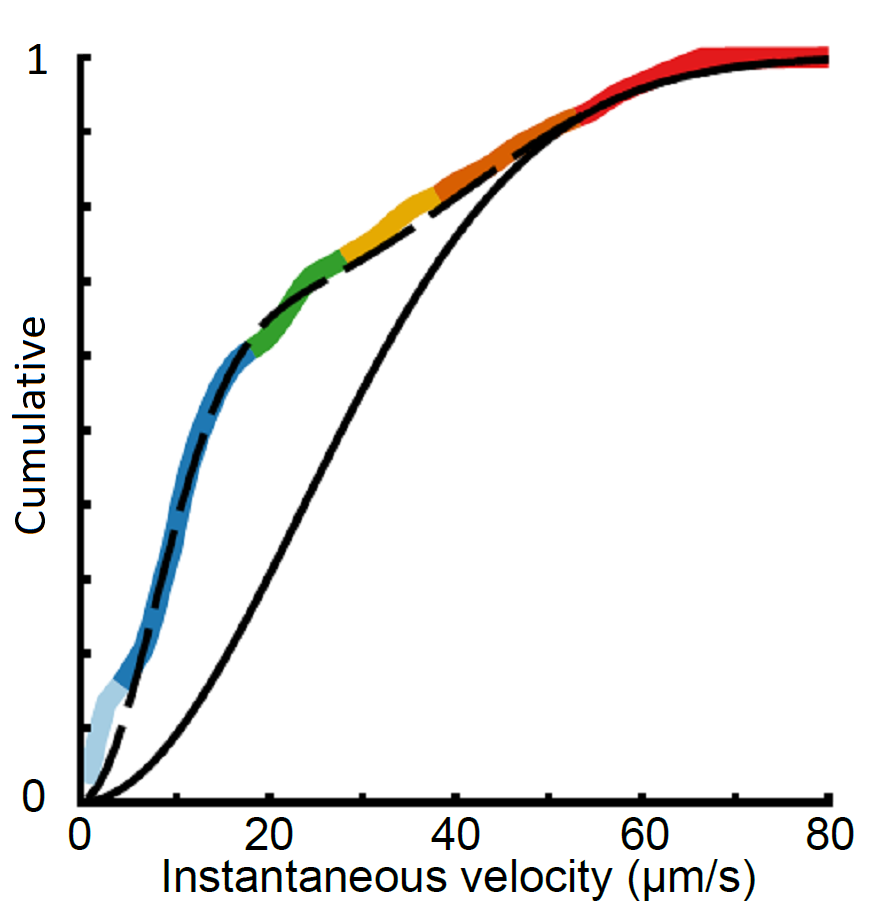
\includegraphics[width=1.0\textwidth]{er-directed-flow-cumulative}
		\caption{} \label{fig:er-directed-flow-cumulative}
	\end{subfigure}
\caption[ER: Single particle tracking reveals directed flow in ER tubules]{(a) shows tracks of single particles in the ER, colour-coded according to the scale in (b) and (c). Fast, directed movement occurs in tubules, and slow movement occurs in nodes. A diffusive model, shown by the solid black line in (b) and (c) does not fit the distribution of velocities; a much better fit is provided using a model which combines directed and diffusive flow, shown by the dashed line. Cell culture and staining was performed by Edward Avezov, and single particle tracking by David Holcman. Graphs were created from n = \num{80563} tracks. }
\label{fig:ER-directed-flow-velocity}
\end{figure}

Figure~\ref{fig:er-directed-flow-distribution} shows that applying data from \num{80563} single particle tracks to a mathematical model with both diffusive and flow terms provided a better fit to experimental data than a model with diffusive motion only.
This is particularly convincing in the cumulative frequency distribution shown in Figure~\ref{fig:er-directed-flow-cumulative}.

Consistent with previous studies~\cite{nehls2000dynamics}, tracking directed flow revealed that depleting ATP causes a 4$\times$ decrease in mean flow velocity, shown in Figure~\ref{fig:er-atp-depletion}.

\begin{figure}[t!]
	\centering
	\begin{subfigure}[b]{0.3\textwidth}
		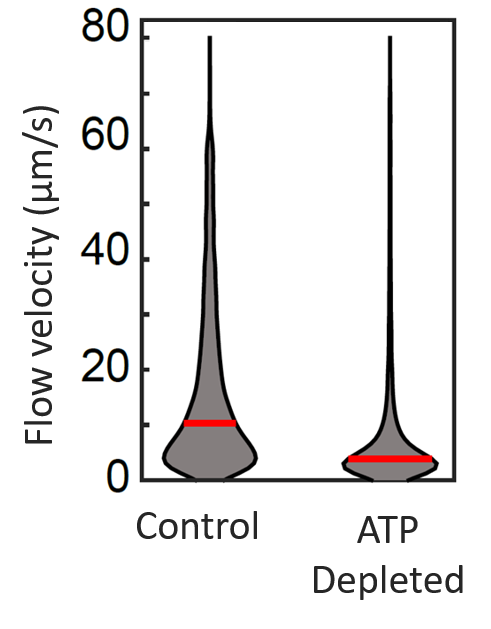
\includegraphics[width=1.0\textwidth]{er-atp-depletion}
		\caption{} \label{fig:er-atp-depletion}
	\end{subfigure}
	\hspace{0.15\textwidth}
	\begin{subfigure}[b]{0.3\textwidth}
		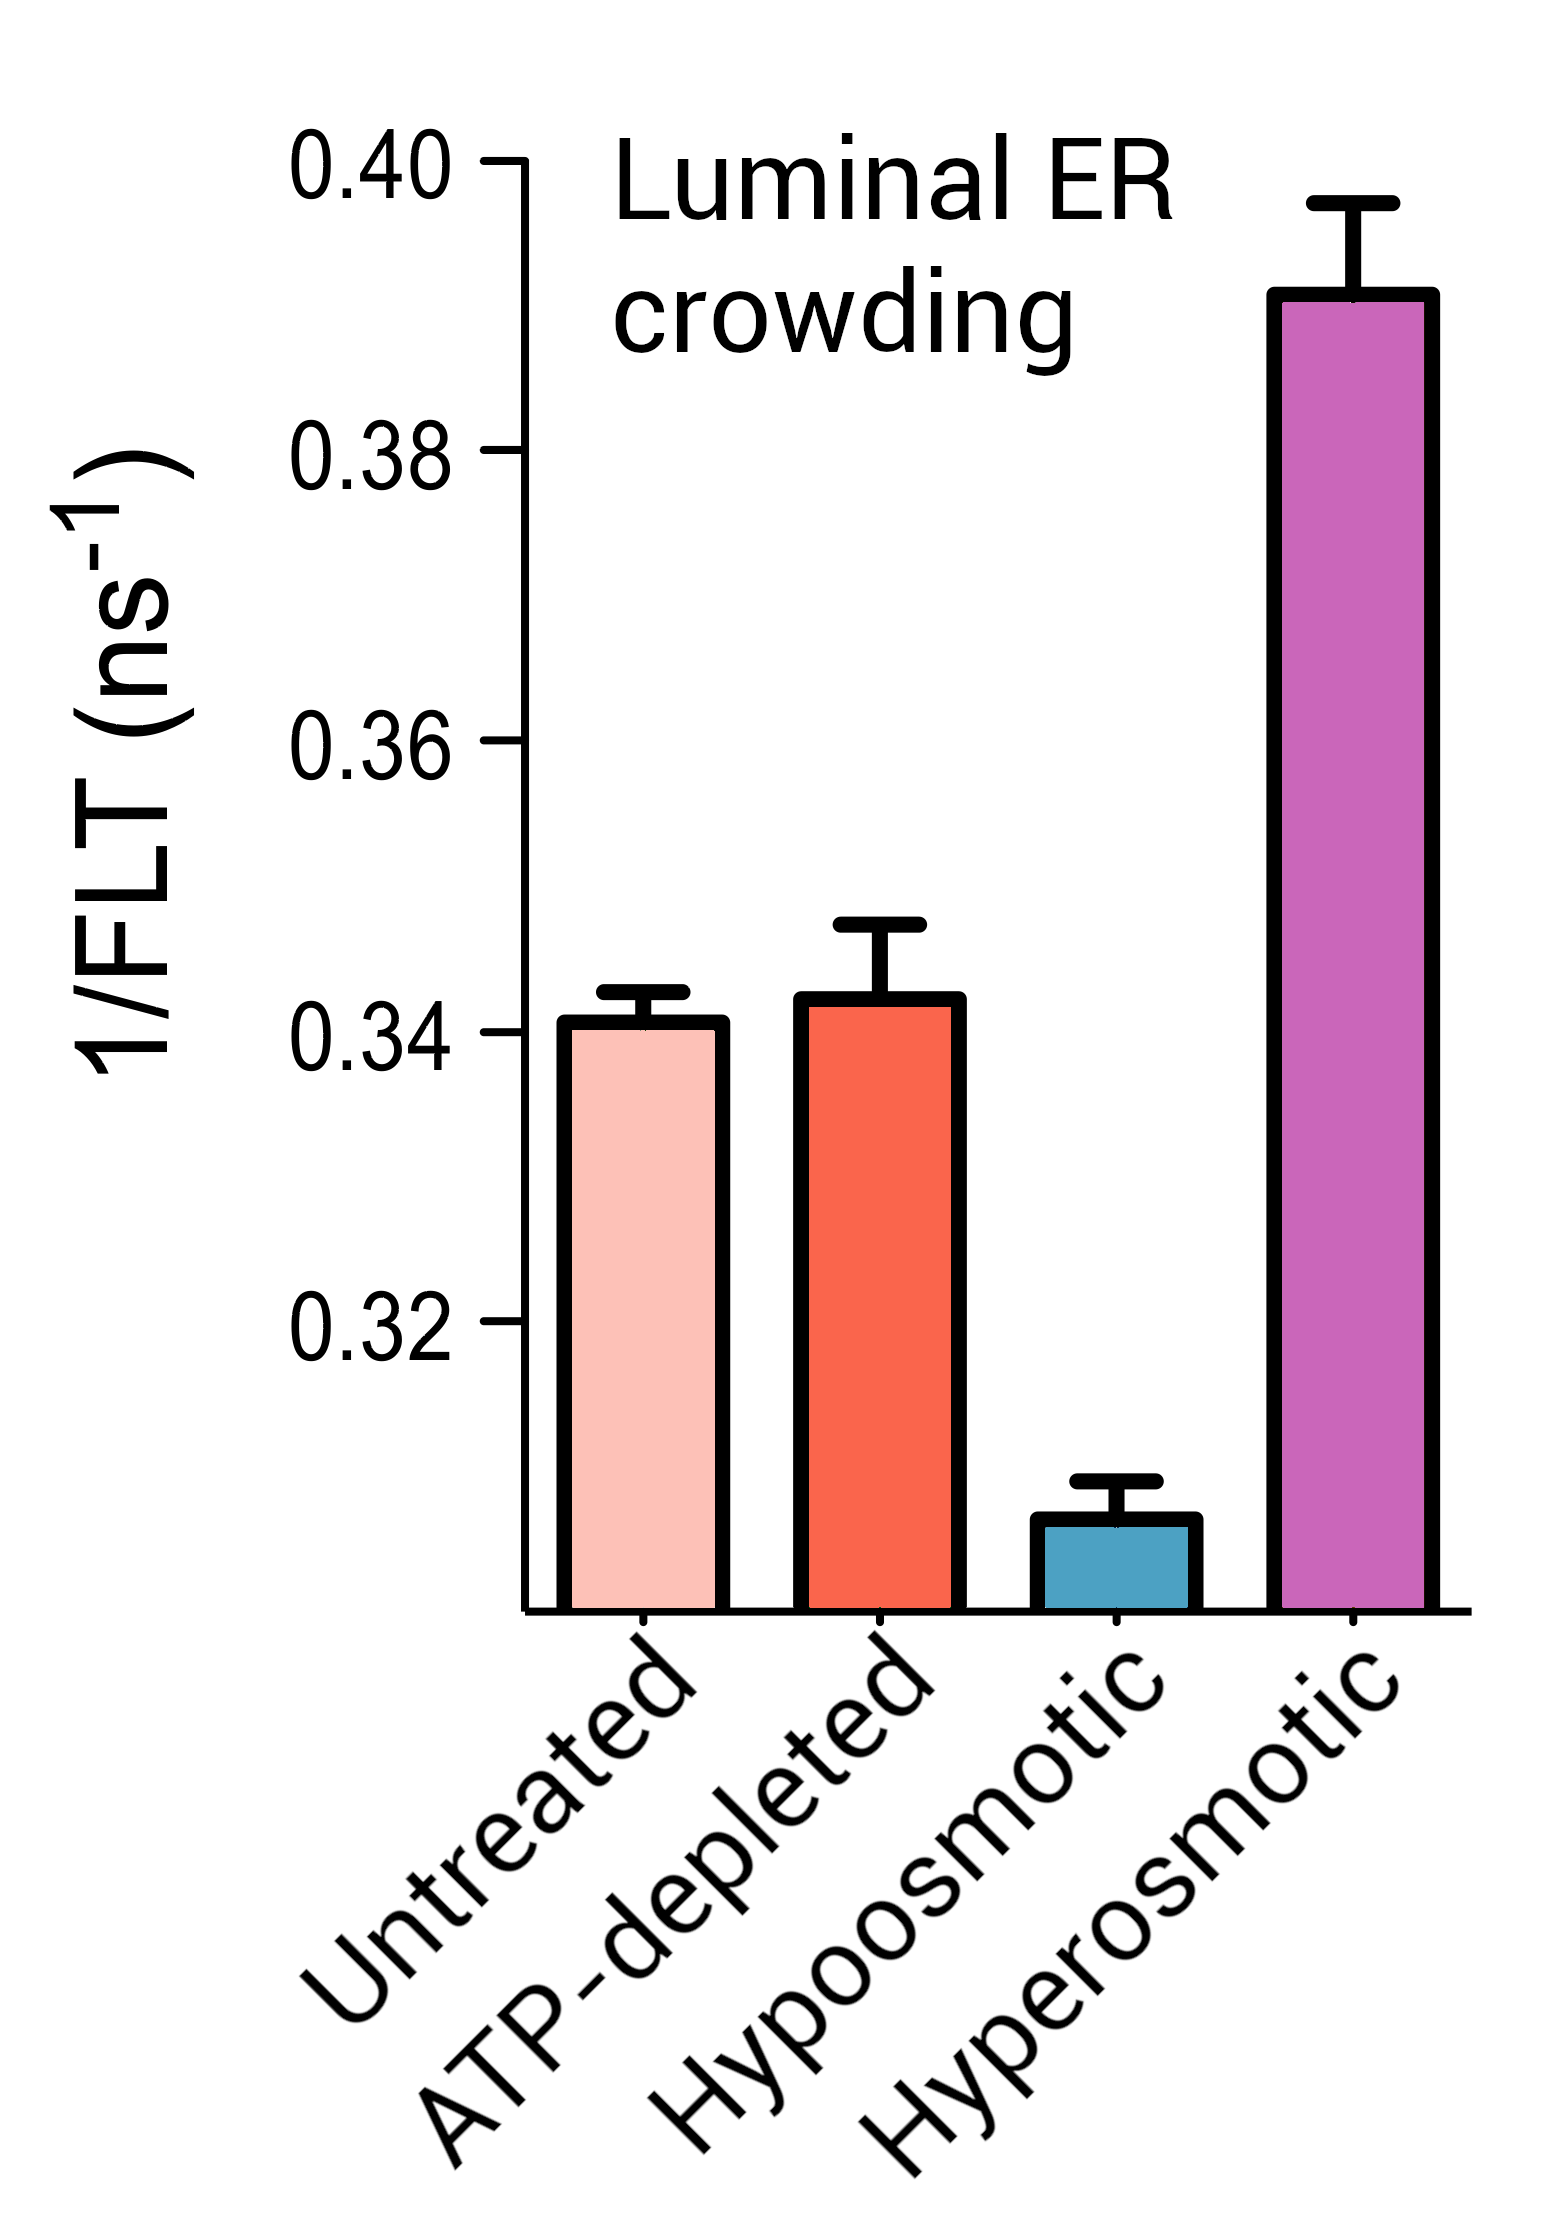
\includegraphics[width=1.0\textwidth]{er-fret-probe}
		\caption{} \label{fig:er-fret-probe}
	\end{subfigure}
	\caption[ER: Flow velocity is reduced upon ATP depletion; a FRET probe reveals this is not due to increased crowding]{(a) shows that mean flow velocity decreased 4$\times$ when ATP was depleted from the cell. A FRET probe was used to assess crowding of luminal ER proteins, shown in (b). Although hypoosmotic conditions caused a decrease in crowding and hyperosmotic conditions caused an increase in crowding, due to expansion and contraction of the cell size respectively, depleting ATP did not change crowding of luminal proteins, countering the argument that a decrease in flow velocity is due to crowding of proteins. Measurements were performed by Edward Avezov. }
	\label{fig:er-atp}
\end{figure}

It was suggested that the decrease in protein mobility could be explained by an increase in the resistance to motion due to crowding of luminal ER proteins.
To counter this argument, a FRET-based probe was used to measure ER crowdedness.
Treating with a hyperosmotic buffer induces cell shrinking, which increases crowding, decreasing the fluorescence lifetime.
Conversely, a hypoosmotic buffer induces cell swelling, decreasing crowding, and the fluorescence lifetime of our sensitive FRET probe increases.
When depleting ATP, there is no change in lifetime;
therefore we dismiss the hypothesis that the change in protein mobility is due to increased crowdedness, but relies on an active, ATP-dependent mechanism.
Further details on the FRET probe implementation and analysis are provided in Appendix~\ref{appn:fret}. 

\subsection{Structure of this chapter}
As part of a collaboration with David Holcman and Edward Avezov, the authors who first observed directed ER flow, I investigated potential mechanisms for flow.
Utilising the unique capabilities of structured illumination microscopy (SIM) and computational analysis, evidence is presented in this chapter that ER luminal flow is caused by pinching of the ER membrane.

The results and methods section which follows details 3 key contributions which I personally made to the published study:
\begin{enumerate}
	\item Measuring dynamic network arrangement with SIM imaging and computational analysis
	\item Imaging tubule pinching with TIRF-SIM and extracting statistics regarding pinching frequency
	\item Computational simulation of tubule pinching to investigate its biological advantage over diffusive transport
\end{enumerate}

Conclusions and future work extending the findings presented here are given at the end of the chapter.
Background invesitgation which I did not personally perform is shown in Appendix B, and further details of the full study can be found in \textit{Nature Cell Biology}~\cite{holcman2018single}.

\section{Results and methods} \label{sec:ERresults}
\subsection[High-speed SIM and image analysis reveals a dynamic ER network]{High-speed SIM and image analysis reveals a dynamic ER\\ network} \label{sec:ERnetwork}
Utilising the high-speed imaging capability of the LAG SIM, we  observed that the ER is a dynamic network, with nodes and tubular endpoints constantly moving to rearrange the network.
Imaging was performed at a raw frame rate of \SI{99}{\hertz}, corresponding to a reconstructed frame rate of \SI{11}{\hertz}.

For optimal imaging conditions, COS-7 cells were selected for the investigation.
These characteristically flat cells, with a height of <\SI{10}{\micro\meter},
meant that the whole ER network could be imaged by LAG SIM in TIRF mode, which physically removes out-of-focus light.
The ER network was labelled with ER-Tracker\textsuperscript{TM} Green, a fluorescent dye from ThermoFisher excited at \SI{488}{\nano\meter}.
This allowed SIM to achieve its highest resolution imaging of \SI{80}{\nano\meter}.

To verify our observations, and ensure relevance to human pathology, we also used HEK-293 cells labelled with tetramethylrhodamine (TMR) attached to luminal ER proteins with HaloTag® technology.
These thicker cells were imaged with optical sectioning LAG SIM, since TIRF only showed small fragments of ER close the coverglass.
Images in this chapter are described as COS-7-ERT, COS-7-TMR, and HEK-293-ERT, and HEK-293-TMR to describe COS-7 and HEK-293 cells labelled with ER-Tracker\textsuperscript{TM} Green or TMR respectively.

\begin{figure}[b!]
\centering
\begin{subfigure}[b]{0.325\textwidth}
	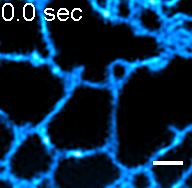
\includegraphics[width=\textwidth]{er-rearrangement-1}
	\caption{}\label{fig:er-rearrangement-1}
\end{subfigure}\hfill
\begin{subfigure}[b]{0.325\textwidth}
	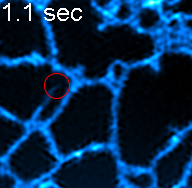
\includegraphics[width=\textwidth]{er-rearrangement-2}
	\caption{}\label{fig:er-rearrangement-2}
\end{subfigure}\hfill
\begin{subfigure}[b]{0.325\textwidth}
	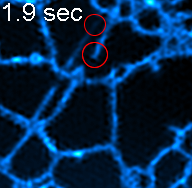
\includegraphics[width=\textwidth]{er-rearrangement-3}
	\caption{}\label{fig:er-rearrangement-3}
\end{subfigure}
\caption[ER: Growing and shrinking tubules show the ER network is in a state of dynamic equilibrium]{The ER network is in a state of dynamic equilibrium, with a small number of nodes being created and destroyed at any given time to cause network rearrangement. Images are of COS-7-ERT; note that these images are a selection from a more detailed timelapse, and these examples are not evenly spaced. Scalebar is \SI{1}{\micro\metre}. }
\label{fig:ER-rearrangement}
\end{figure}

Figure~\ref{fig:ER-rearrangement} shows a small area of the ER network in COS-7-ERT cells.
The network's tubules and nodes are clearly visible, as well as large and small loops in the network and sheet structures.
The time series shows that the ER network undergoes fast rearrangements, with a number of tubules growing and shrinking and nodes rearranging at any given time.
The speed of this process highlights the need for the fast, high-resolution imaging technique provided by LAG SIM.

To draw statistics describing the network from the images, the following steps were performed:
\begin{enumerate}
	\item Generate a binary image of the network for each frame
	\item Skeletonise the network, making it one pixel wide
	\item Classify nodes, endpoints, and tubes with MATLAB's \texttt{bwmorph} functions
	\item Extract statistics from labelled binary image stacks
\end{enumerate}

A common method for generating a binary image is thresholding, where all pixels with a value above a certain threshold are classified as \texttt{true} and all those with values below the threshold are assigned \texttt{false}.
Whilst this scheme was effective at differentiating ER from background in the thin COS-7 cells, non-uniform background light in HEK-293 cells, visible in Figure~\ref{fig:er-classifier-recon-561}, meant that a simple binary threshold produced the poor network extraction shown in Figure~\ref{fig:ER-classifier-threshold}.
Furthermore, the binary threshold required for each image set varies depending on exposure time, laser power, and expression level of the fluorescent label in that particular cell.
Therefore a single value threshold was not appropriate to generate binary images.

Binary morphology was was also considered as a classification technique, where opening and closing operations were performed with line segments and disks respectively. 
Due to the variety of line segment lengths and shapes, however, a repeatable set of operations could not be devised, and structuring elements required time-consuming fine tuning for each image set. 

\begin{figure}[p!]
	\centering
	\begin{subfigure}[b]{0.325\textwidth}
		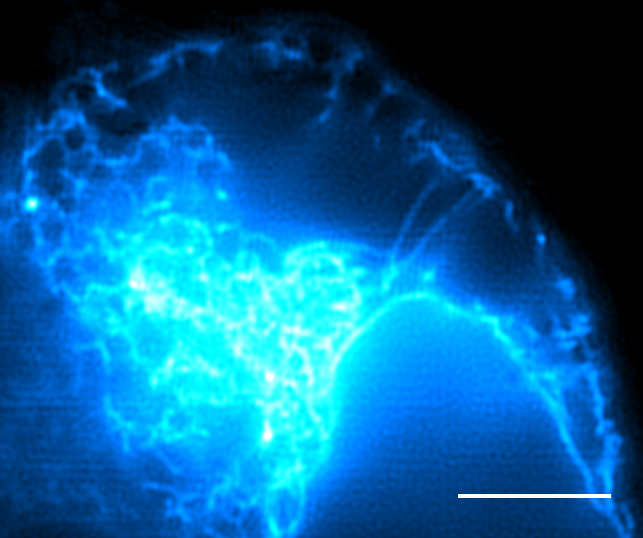
\includegraphics[width=1.0\textwidth]{er-classifier-recon-561}
		\caption{} \label{fig:er-classifier-recon-561}
	\end{subfigure}
	\hfill
	\begin{subfigure}[b]{0.325\textwidth}
		
\includegraphics[width=1.0\textwidth]{er-classifier-threshold}
		\caption{} \label{fig:ER-classifier-threshold}
	\end{subfigure}
	\hfill
	\begin{subfigure}[b]{0.325\textwidth}
		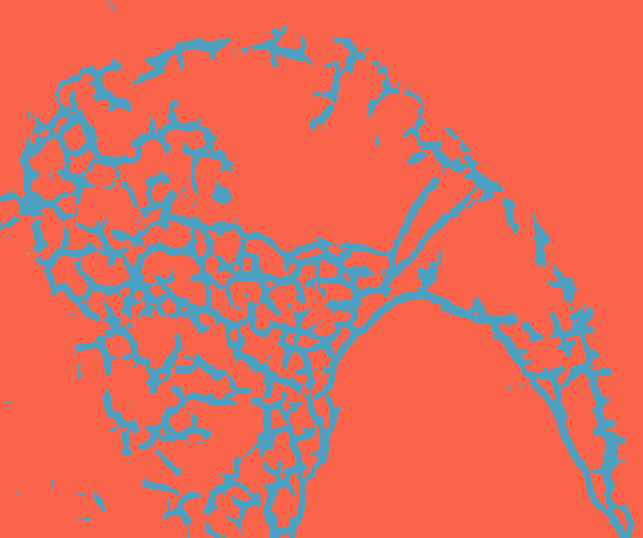
\includegraphics[width=1.0\textwidth]{er-classifier-weka}
		\caption{} \label{fig:ER-classifier-weka}
	\end{subfigure}

	~\newline
	\begin{subfigure}[b]{0.8\textwidth}
		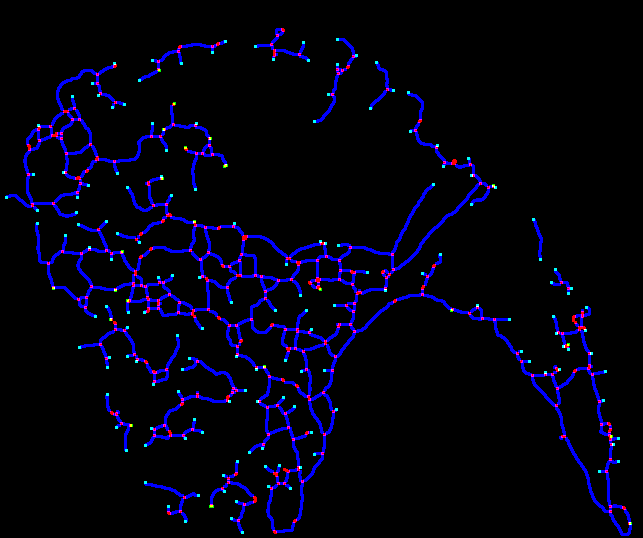
\includegraphics[width=1.0\textwidth]{er-classified-network}
		\caption{} \label{fig:er-classified-network}
	\end{subfigure}
	\caption[ER: Weka segmentation allows the ER network to be extracted from a non-uniform background]{(a) shows a SIM reconstruction of ER where the background is not uniform and honeycomb artefacts have appeared, as described in Section~\ref{sec:sim-artefacts}. A simple threshold for separating ER from the background, shown in (b), does not work well on HEK-293 cells due to the variations in background intensity. A machine learning technique, implemented with the Weka segmentation plugin for ImageJ, identifies the ER and background more reliably, as shown in (b). A MATLAB script was applied to the binary image to classify ER tubes, nodes, and end-points, labelled in (d) as blue, green, and red respectively. Tracking of nodes and endpoints, and analysis of tubule length distribution, could then be performed on the network. Images are of HEK-293-ERT; scalebar is \SI{5}{\micro\metre}. }
	\label{fig:ER-classifier}
\end{figure}

Instead a machine learning technique was used to classify ER pixels from background pixels.
Using the Trainable Weka Segmentation plugin for ImageJ~\cite{arganda2017trainable}, a set of training data was generated by manually classifying ER pixels and background pixels.
The Adaboost algorithm was used to quickly refine the classification~\cite{freund1997decision, schapire1999brief}, leading to a reliable and automated adaptive thresholding method.
The output of Weka Segmentation in Figure~\ref{fig:ER-classifier-weka} successfully extracts the ER network even with the unideal imaging properties of HEK-293 cells.

After binary images were skeletonised, a classified network map, as shown in Figure~\ref{fig:er-classified-network}, was generated with MATLAB for every frame of every image set.
From this, various statistics could be extracted, including tubule length distribution, tip growth rate, and node movement.

The distribution of tubule lengths, shown at various time points in Figure~\ref{fig:er-tubule-timepoints}, does not change over time.
This shows that the ER is in a dynamic equilibrium.
Although there are local changes in structure and connectivity, the overall network properties do not change.

\begin{figure}[b!]
\centering
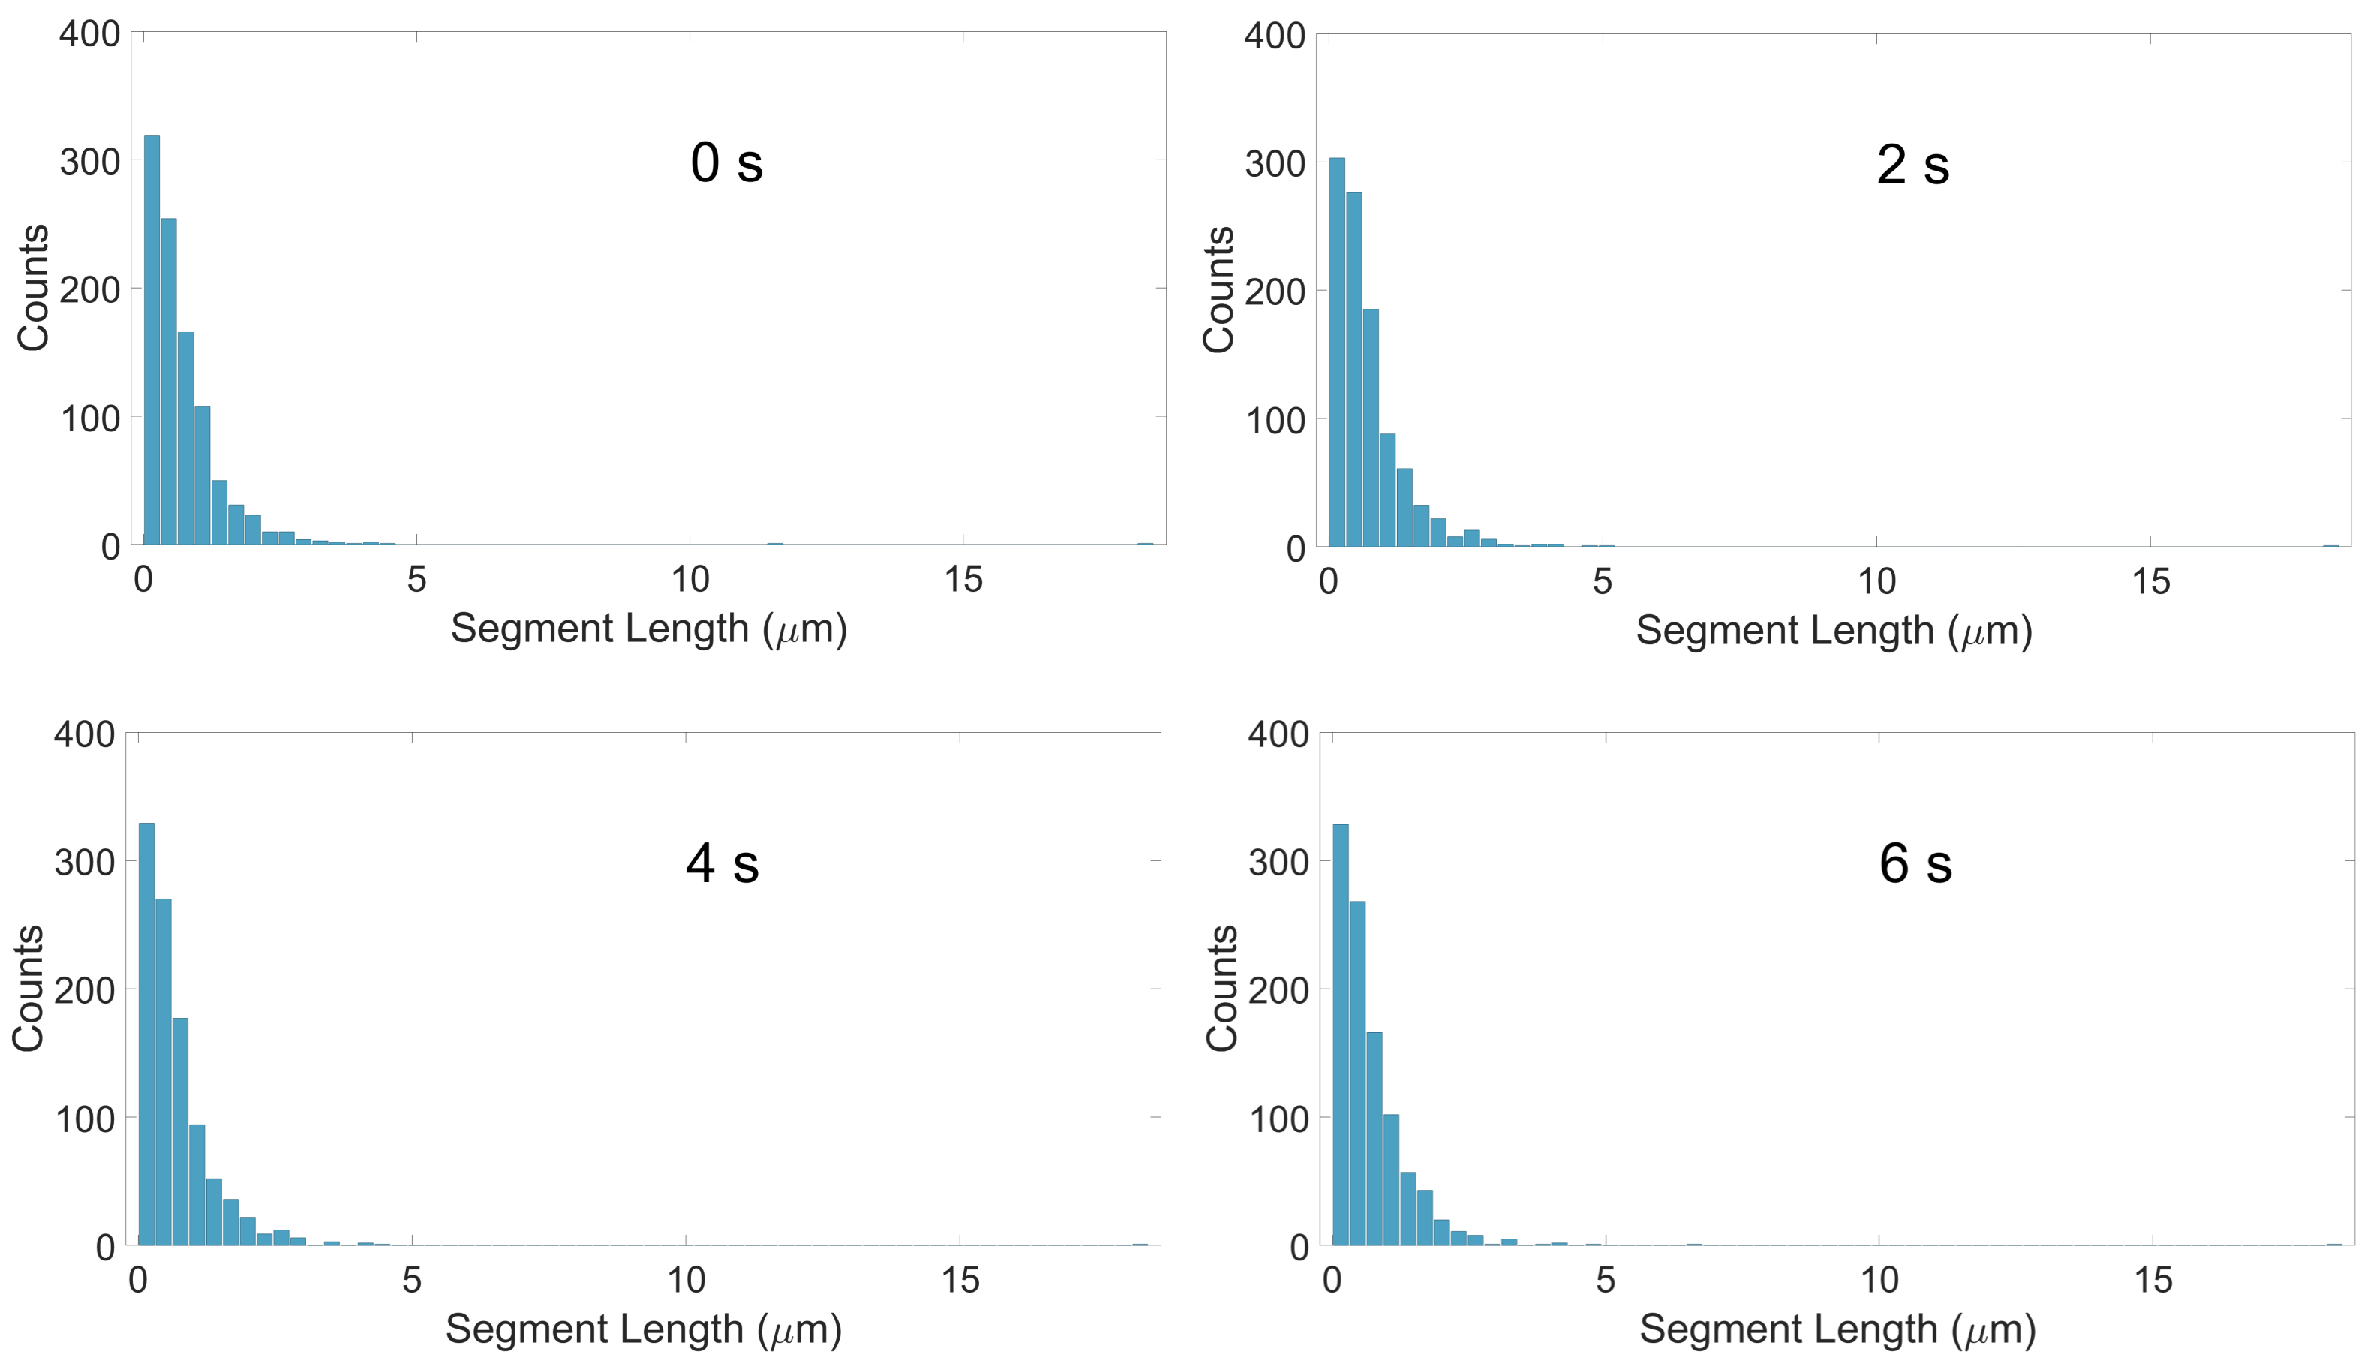
\includegraphics[width=1.0\textwidth]{er-tubule-timepoints}
\caption[ER: Distribution of tubule length remains constant despite growing and shrinking of individual tubules]{Although individual tubules are growing and shrinking at any given time, as shown in Figure~\ref{fig:ER-rearrangement}, the distribution of tubule lengths does not vary over time, showing that the ER is in a dynamic equilibrium. }
\label{fig:er-tubule-timepoints}
\end{figure}

Movement of end points and nodes was initially suggested as a hypothesis for the distribution of particle movement inside the ER.
However tracking of nodes revealed an average speed of just \SI[separate-uncertainty=true]{0.39 \pm 0.42}{\micro\metre\per\second}, around 60$\times$ slower than the \SI{22.9}{\micro\metre\per\second} mean speed of particles found in the single particle tracking analysis of Figure~\ref{fig:er-directed-flow-distribution}.
Furthermore, we calculated that just \SI[separate-uncertainty=true]{0.14 \pm 0.04}{\percent} of tubules were growing at any given time.
We conclude that tubule growth and node movement have a negligible contribution to particles' diffusion and flow velocities.

%Experiments are now underway to understand the biochemistry behind network rearrangement, which is described in more detail in the Future Work Section~\ref{sec:ERfuture}.

\subsection{Active tubule pinching correlates with luminal flow velocity}
The motion of luminal proteins suggested the possibility of nanoperistalsis-like propulsion~\cite{nadeem2014mathematical}, attainable by tubule contractions.
Using the LAG SIM in TIRF mode, we obtained images at \SI{11}{\hertz}, with a resolution of \SI{80}{\nano\metre}, and were able to observe pinching of the tubule.

ER tubules are \SIrange{60}{100}{\nano\metre} in width, so observing pinching requires a microscope that can image beyond the diffraction limit~\cite{lippincott1989rapid}.
When ER tubules pinch, their width decreases to below the resolution limit of SIM; however this can still be observed as a decrease in intensity, confirmed by the simulation shown in Figures~\ref{fig:er-pinching}a-f.

\begin{figure}[tbp]
\centering
\begin{subfigure}[b]{0.16\textwidth}
	
\includegraphics[width=\textwidth]{pre-pinch-full}
	\caption{}\label{fig:pre-pinch-full}
\end{subfigure}\hfill
\begin{subfigure}[b]{0.16\textwidth}
	
\includegraphics[width=\textwidth]{pinched-full}
	\caption{}\label{fig:pinched-full}
\end{subfigure}\hfill
\begin{subfigure}[b]{0.16\textwidth}
	
\includegraphics[width=\textwidth]{pre-pinch-blur}
	\caption{}\label{fig:pre-pinch-blur}
\end{subfigure}\hfill
\begin{subfigure}[b]{0.16\textwidth}
	
\includegraphics[width=\textwidth]{pinched-blur}
	\caption{}\label{fig:pinched-blur}
\end{subfigure}\hfill
\begin{subfigure}[b]{0.16\textwidth}
	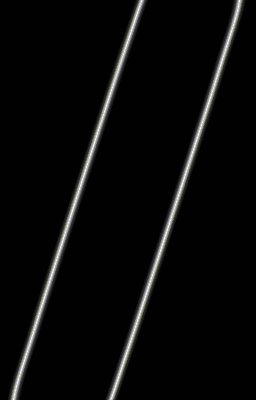
\includegraphics[width=\textwidth]{pre-pinch-edges}
	\caption{}\label{fig:pinched-edges}
\end{subfigure}\hfill
\begin{subfigure}[b]{0.16\textwidth}
	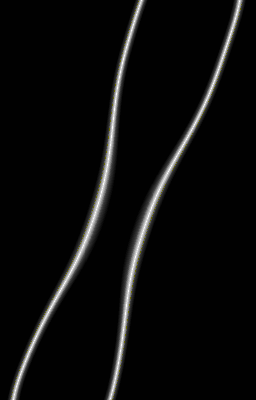
\includegraphics[width=\textwidth]{pinched-edges}
	\caption{}\label{fig:pre-pinch-edges}
\end{subfigure}

~\newline
\begin{subfigure}[b]{0.36\textwidth}
	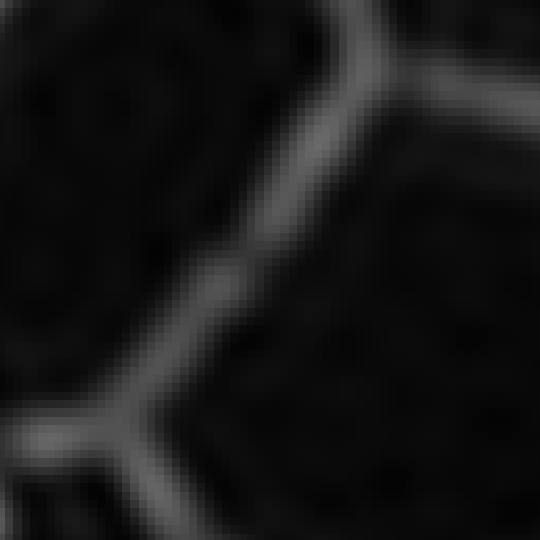
\includegraphics[width=\textwidth]{pinch-real}
	\caption{}\label{fig:pinched-real}
\end{subfigure}\hfill
\begin{subfigure}[b]{0.36\textwidth}
	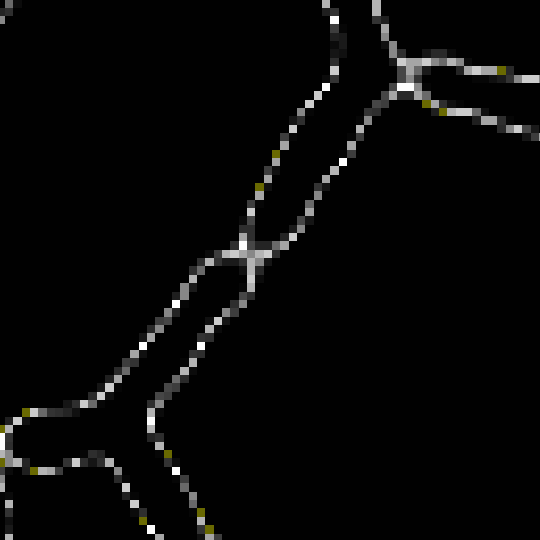
\includegraphics[width=\textwidth]{pinch-real-edges}
	\caption{}\label{fig:pre-real-edges}
\end{subfigure}\hfill
\begin{subfigure}[b]{0.265\textwidth}
	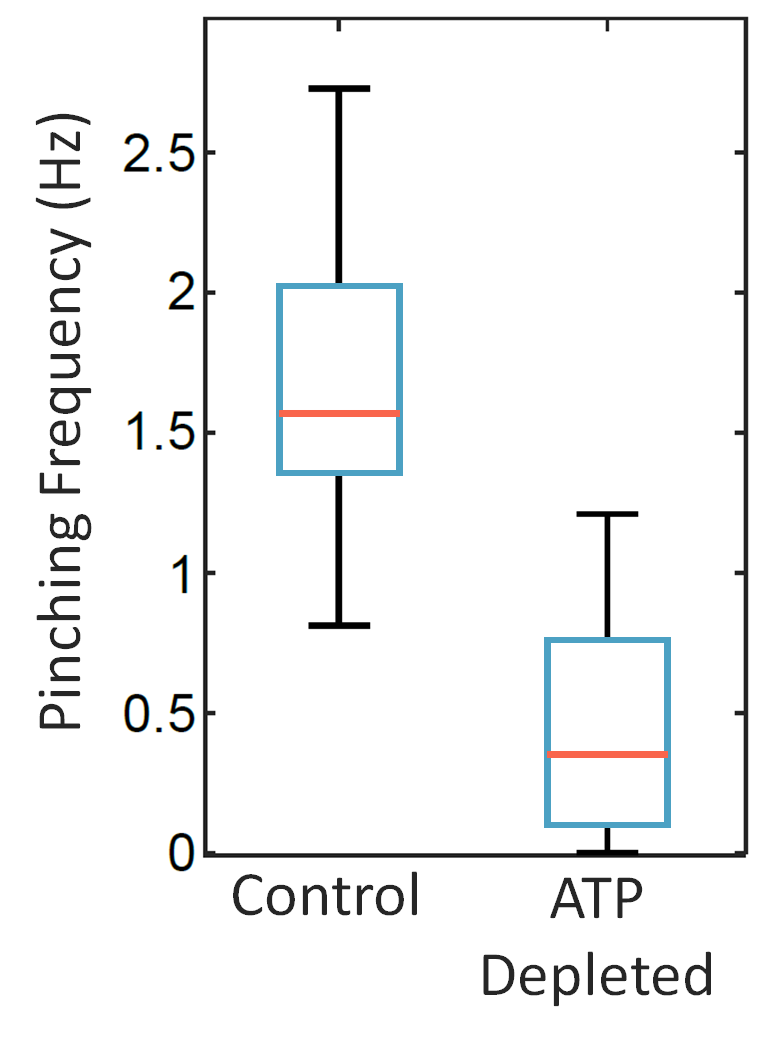
\includegraphics[width=\textwidth]{pinching-atp-depletion}
	\caption{}\label{fig:pinching-atp-depletion}
\end{subfigure}
\caption[ER: Tubule pinching can be observed with the `Edges' colourmap]{A simulation in (a-f) shows that pinching events can be observed even when the pinch width is below the resolution limit of SIM. (a) and (b) show an unpinched and pinched tubule at full simulation resolution, with a width of \SI{80}{\nano\metre}. (c) and (d) show the tubule after convolution with a SIM-resolution point-spread function; (e) and (f) show that using the `Edges' colourmap clearly shows the pinch.  (g) shows experimental data of a tubule pinching in COS-7-ERT cells, highlighted in (h) by the `Edges' colourmap. (i) shows that ATP depletion reduces pinching frequency 3.9$\times$, with a similar dependence on ATP as luminal flow velocity seen in Figure~\ref{fig:er-atp-depletion}. }
\label{fig:er-pinching}
\end{figure}

To clearly visualise pinches, the `Edges' colourmap was used in ImageJ, highlighting lines of constant intensity.
Note that, whilst this allows pinching events to be accurately counted, there is not enough resolution in SIM to measure the width of the tubule when it is pinched.
Nevertheless we believe that SIM is still the only technique capable of capturing these dynamic events, due to its combination of spatial resolution and imaging speed.

Counting the number of pinches in each tube over time gave the mean frequency of pinches as \SI[separate-uncertainty=true]{1.70 \pm 0.48}{pinches\per\second} in COS-7 cells.
Figure~\ref{fig:pinching-atp-depletion} shows that when ATP was depleted, the frequency decreased 3.9$\times$, to \SI[separate-uncertainty=true]{0.44 \pm 0.41}{pinches\per\second}.
This decrease in pinching frequency is very similar to the velocity decrease observed with single particle tracking in Figure~\ref{fig:er-atp-depletion}, suggesting that there is a strong link between tubule pinching and directed motion in the ER.

\begin{figure}[b!]
\centering
\begin{subfigure}[b]{0.325\textwidth}
	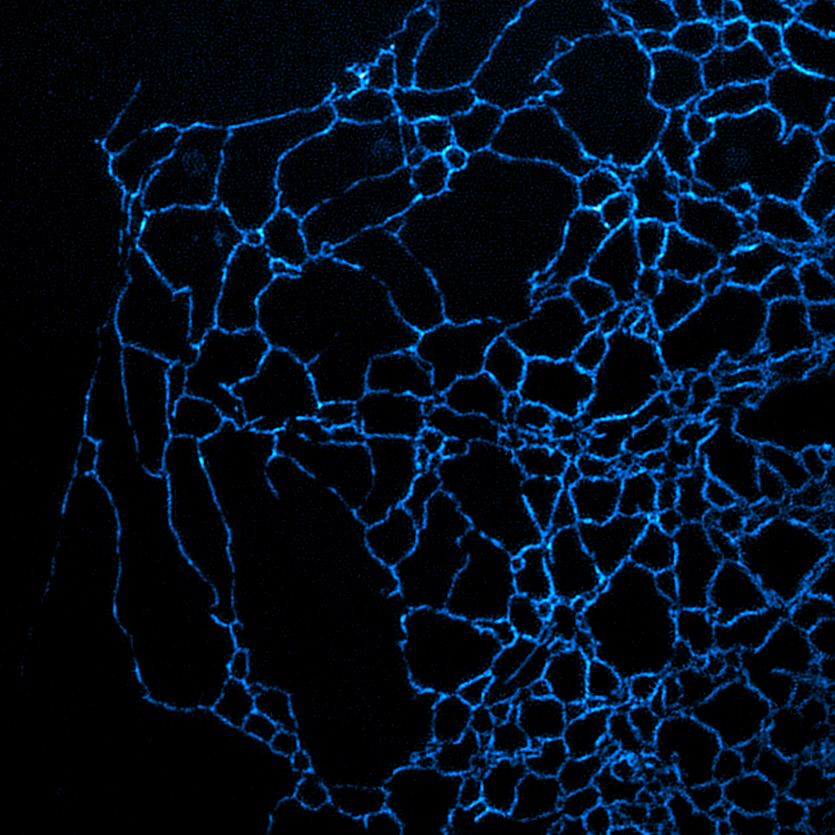
\includegraphics[width=\textwidth]{er-blebbing-1}
	\caption{}\label{fig:er-blebbing-1}
\end{subfigure}\hfill
\begin{subfigure}[b]{0.325\textwidth}
	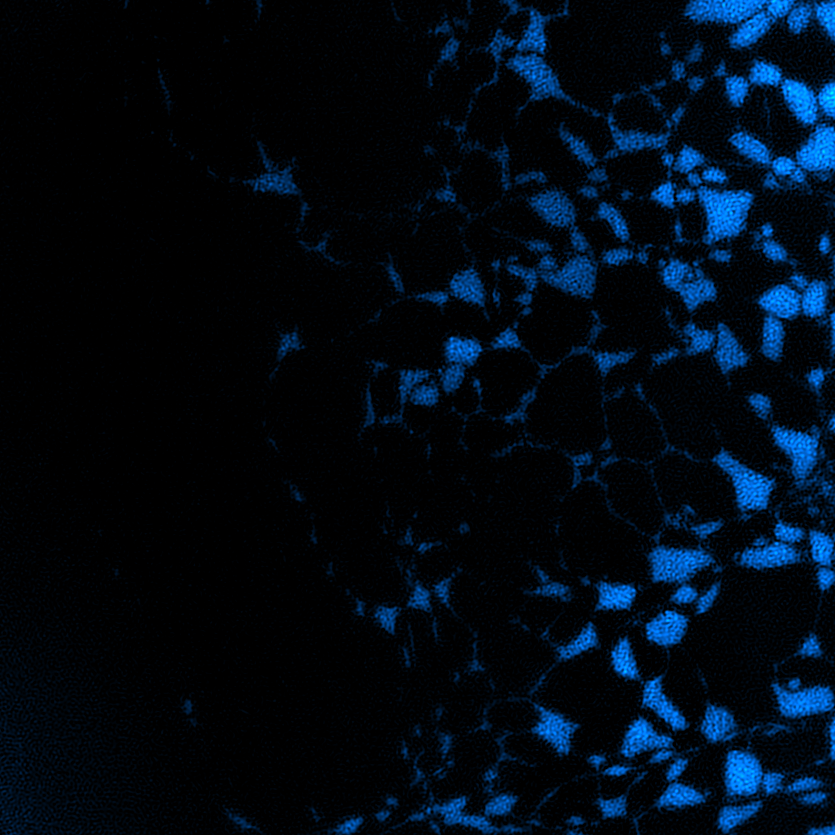
\includegraphics[width=\textwidth]{er-blebbing-2}
	\caption{}\label{fig:er-blebbing-2}
\end{subfigure}\hfill
\begin{subfigure}[b]{0.325\textwidth}
	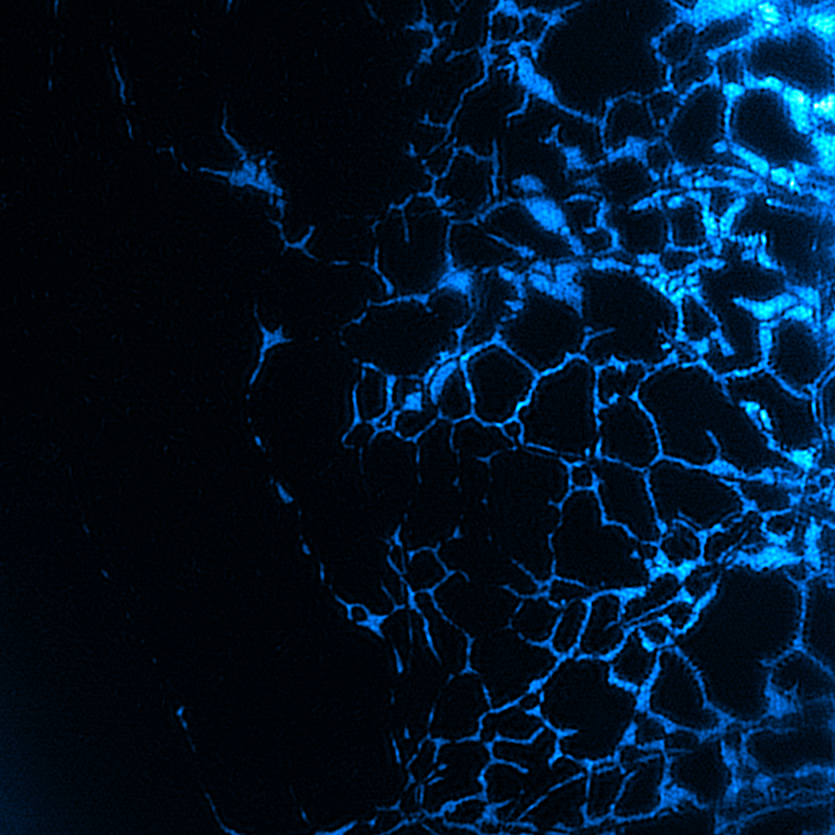
\includegraphics[width=\textwidth]{er-blebbing-3}
	\caption{}\label{fig:er-blebbing-3}
\end{subfigure}
\caption[ER: Phototoxicity confirms the ability of ER to undergo reversible pinching]{When the cell shown in (a) is strongly perturbed from normal conditions, for example by phototoxicity or calcium manipulation, extreme pinching causes blebbing in the ER. (b) shows the cell after imaging for \SI{30}{\second} with \SI{50}{\watt\per\cm\squared} \SI{561}{\nano\metre} laser light. When the perturbation is removed, the ER recovers its normal shape; (c) shows the same cell after \SI{10}{\minute} of recovery time. This experiment confirms the ability of ER to undergo reversible pinching. }
\label{fig:ER-blebbing}
\end{figure}

Further evidence for tubule pinching was gathered when the cell was artificially placed under excessive stress.
Whilst acquiring time series videos of the ER on the LAG SIM, we occasionally observed a reversible blebbing behaviour of the ER.
This phenomenon, shown in Figure~\ref{fig:ER-blebbing}, was particularly evident when imaging samples labelled with TMR fluorescent dye with the \SI{561}{\nano\meter} laser power set to \SI{95}{\milli\watt} or more, equivalent to \SI{50}{\watt\per\cm\squared} at the sample.
The same behaviour was observed when calcium manipulation~\cite{subramanian1997calcium} was performed on the cell.
Notably, the ER recovers its original shape after the stress is removed, demonstrating the ability of ER tubules to undergo reversible pinching.

Furthermore, 3D images of a fixed ER network, obtained using optical sectioning SIM, reveal tubules pinched in 3D.
This is available to view interactively with FPBioimage, at \url{https://fpb.ceb.cam.ac.uk/ER}.
Despite tubules' size being at the resolution limit of SIM, the evidence from the different experiments presented here provide confidence that pinching is not an imaging artefact.

\subsection{Graphical simulation shows pinching accelerates luminal mixing}
In order to visualise the concept of luminal flow, and to understand its purpose, I wrote a 2D Unity program modelling an ER network with labelled proteins.

An ER network was automatically modelled with the following steps:
\begin{enumerate}
	\item Create binary image of ER network, with method outlined in Section~\ref{sec:ERnetwork}
	\item Create a collision boundary from binary image with an edge-tracing algorithm
	\item Create a simplified skeleton network from binary image
	\item Spawn `pinch points' on the skeleton, aligned with the skeleton direction and the width of the network at that point
\end{enumerate}
The program will accept any binary network image as an input, and will perform these steps automatically using custom C\# implementations of the Moore-Neighbourhood tracing algorithm for tracing tubule edges~\cite{moore-neighbourhood}, the Zhang-Suen algorithm for skeletonisation~\cite{zhang1984fast}, and the Ramer–Douglas–Peucker algorithm for simplifying the tubule skeleton and edges~\cite{ramer1972iterative, douglas1973algorithms}.

Dynamics are modelled in the network at a particle level.
Each particle which is spawned in the network has a physics script attached to it controlling its diffusive motion and its flow velocity when in the vicinity of a pinch.

Diffusive motion was modelled as Brownian motion~\cite{einstein1905molekularkinetischen}.
After travelling a random distance, sampled from a distributed centred on the mean free path, particles randomly change direction as though collided into by an invisible particle~\cite{lucretius1631}.
Diffusion properties are set in the simulation with two of either mean free path $\delta$, time between collisions $\tau$, mean velocity $v$, or the diffusion coefficient $D$, related by $D=\frac{\delta^2}{2\tau}=\frac{v\delta}{2}$~\cite[\textit{ch. 19}]{fishbane1998physics}.

Pinching of the ER tubules simulated a force on particles in the vicinity of the pinch point.
As the tubule contracts, this force acts away from the pinch, in a direction along the tubule, and decays exponentially over time.
When the pinch point relaxes, the force acts in the opposite direction, sucking particles towards the pinch point.
The magnitude of the force is an adjustable parameter, to control overall energy in the system.

Inelastic collisions were modelled with the Nvidia PhysX engine~\cite{nvidia2008physx}.
Coefficient of restitution can be adjusted for each material, such that a collision with the ER membrane is different to a particle-particle collision.

\begin{figure}[t!]
	\centering
	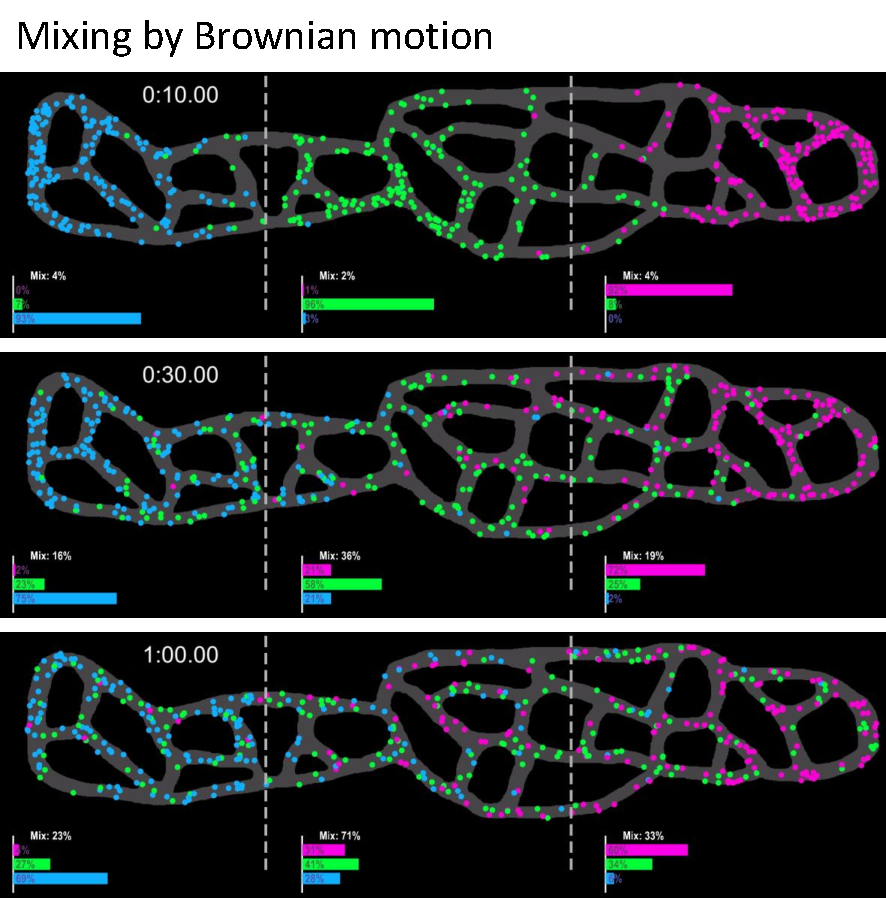
\includegraphics[width=\textwidth]{brownian}
	\caption[ER simulation: After one minute of mixing by Brownian motion the simulated ER mixture is not homogeneous]{After \SI{10}{\second} of mixing by Brownian motion, most particles are still in the third of the network they started in. After \SI{1}{\minute} of mixing, the middle section is 71\% mixed, although the two edge sections are just 23\% and 33\% mixed, showing that particles do not transverse the network quickly under Brownian motion alone. }
	\label{fig:ER-simulation-brownian}
\end{figure}

\begin{figure}[t!]
	\centering
	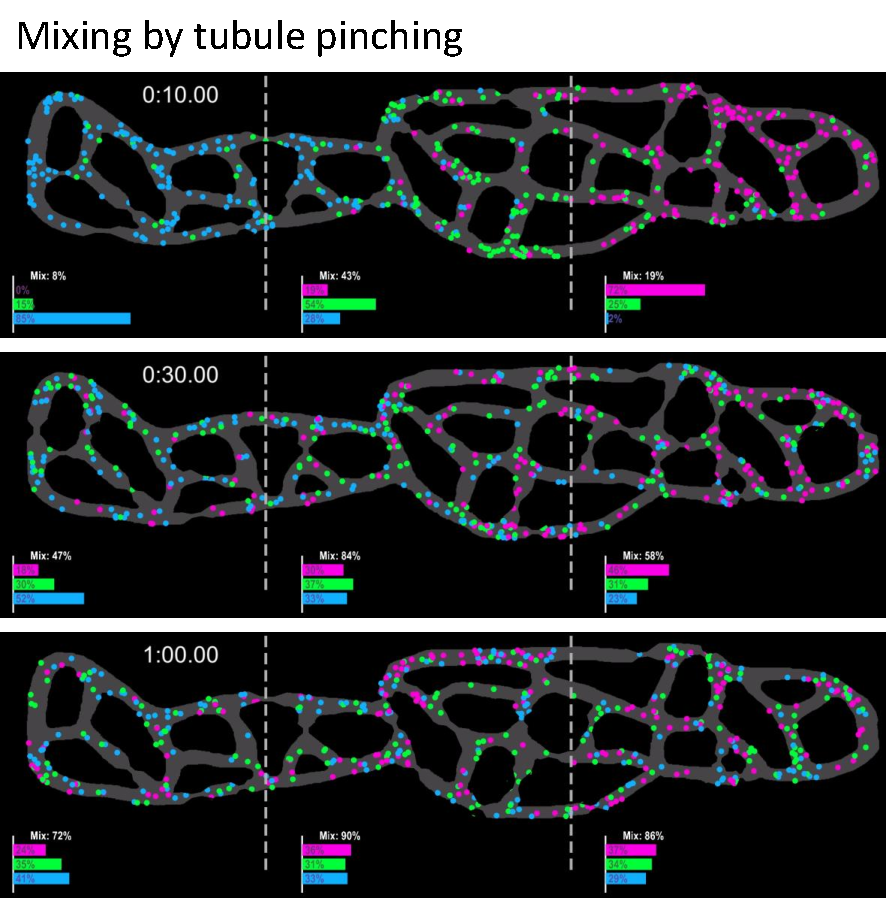
\includegraphics[width=\textwidth]{pinching}
	\caption[ER simulation: A homogeneous mixture is achieved after one minute in the ER simulation with pinching]{When the simulation is executed with tubule pinching, mixing occurs much faster than by Brownian motion despite the same average particle speed.}
	\label{fig:ER-simulation-pinching}
\end{figure}

With this physics model, it was possible to simulate different scenarios to understand experimental observations.
Firstly, the model was executed without any pinching, simulating purely diffusional motion.
In the second scenario, pinching physics was turned on, such that particles in the vicinity of a pinch point experienced a pushing force as the tubule pinched or a pulling force as it relaxed.
The parameters were tuned to ensure an equal mean particle speed in both scenarios for a fair comparison.

The two scenarios were compared by measuring the distribution of particles in the network over time, as shown in Figures~\ref{fig:ER-simulation-brownian} and \ref{fig:ER-simulation-pinching}.
Particles starting at the left hand side of the network were labelled blue; particles in the middle, green; and particles starting on the right pink.
By counting the number of particles in different areas of the network, a quantitative description of network mixing can be obtained.

Comparing Figures~\ref{fig:ER-simulation-brownian} and \ref{fig:ER-simulation-pinching} shows that pinching provides the ER a faster way of moving particles stochastically around the network.
Under Brownian motion alone, after one minute of simulation pink particles which started on the right-hand-side of the network make up just 6\% of particles in the left-hand third of the network.
Conversely with ER pinching dynamics, after one minute pink particles make up 24\% of particles on the left-hand-side.
Pinching dynamics allow particles are able to travel greater distances in the network in less time, even with the same average speed as the diffusional model.

\begin{figure}[b!]
	\centering
	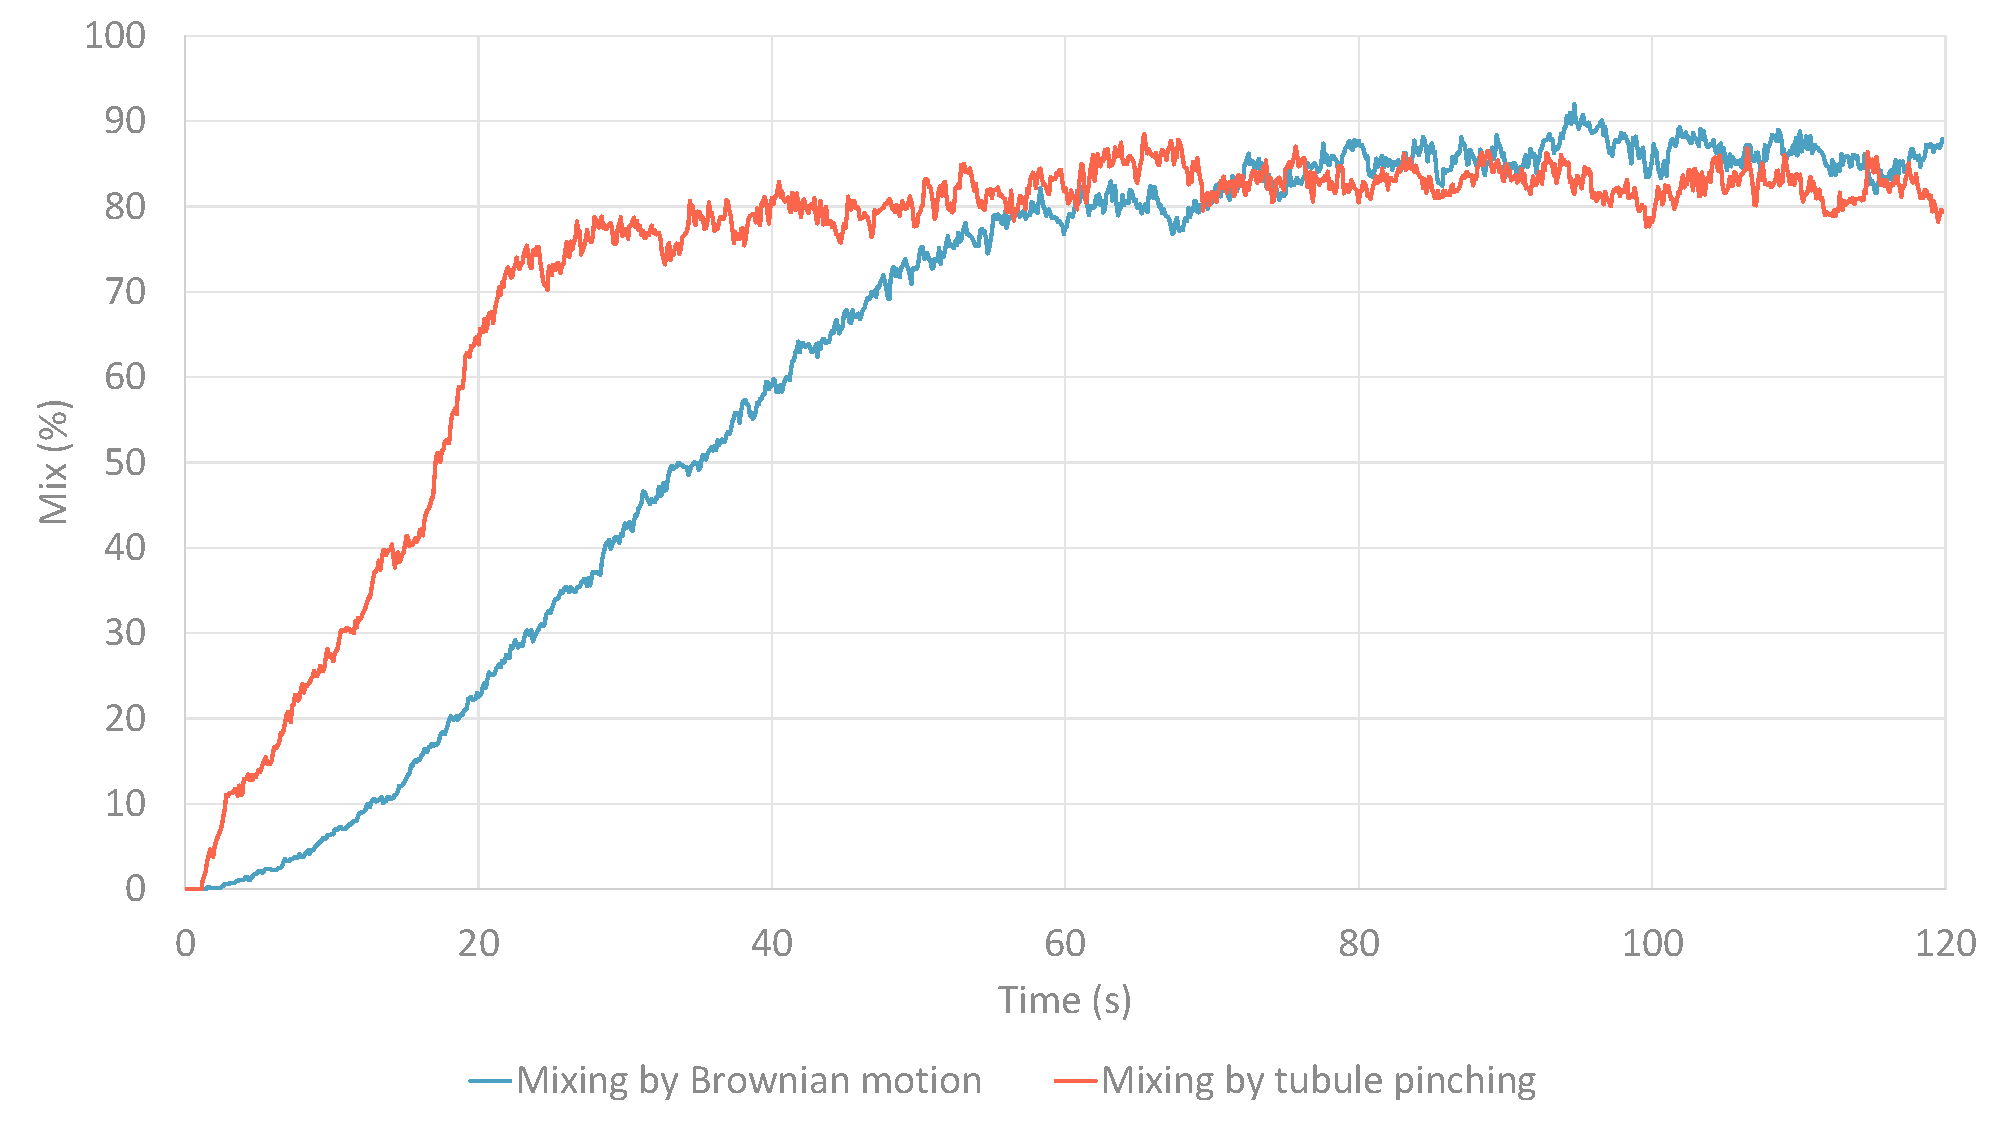
\includegraphics[width=\textwidth]{mixing-over-time-graph}
	\caption[ER simulation: Tubule pinching provides faster mixing than Brownian motion alone]{Mixing percentage for the middle third of the ER simulation was plotted against time for the two conditions. Mixing occurs about 3$\times$ faster with tubule pinching, despite the same average particle speed, allowing particles to reach remote parts of the network faster.}
	\label{fig:mixing-over-time-graph}
\end{figure}

Furthermore, particle motion with ER pinching results in homogeneous mixing in a shorter space of time.
After \SI{30}{\second} of simulation with pinching, the middle section of the graph is 84\% mixed - where mixing percentage is measured as the sum of the second- and third-most abundant particle colour in an area divided by 2$\times$the most abundant particle colour.
At the same timepoint under pure Brownian motion, however, the middle section is only 36\% mixed; and the edge sections even less so.
Figure~\ref{fig:mixing-over-time-graph} shows how mixing in the middle section develops over time; pinching allows mixing to occur 3$\times$ faster than diffusive motion alone.
Overall, particles are mixed faster with ER pinching.

Pinching events are uncoordinated, so that mixing with pinching is stochastic rather directed, which agrees with experimental observations.
Particles gain enough speed from a pinch to move away from its influence when the pinch relaxes, so that particles do not stay stuck in one area but are able to freely mix in the network.

\begin{figure}[t!]
	\centering
	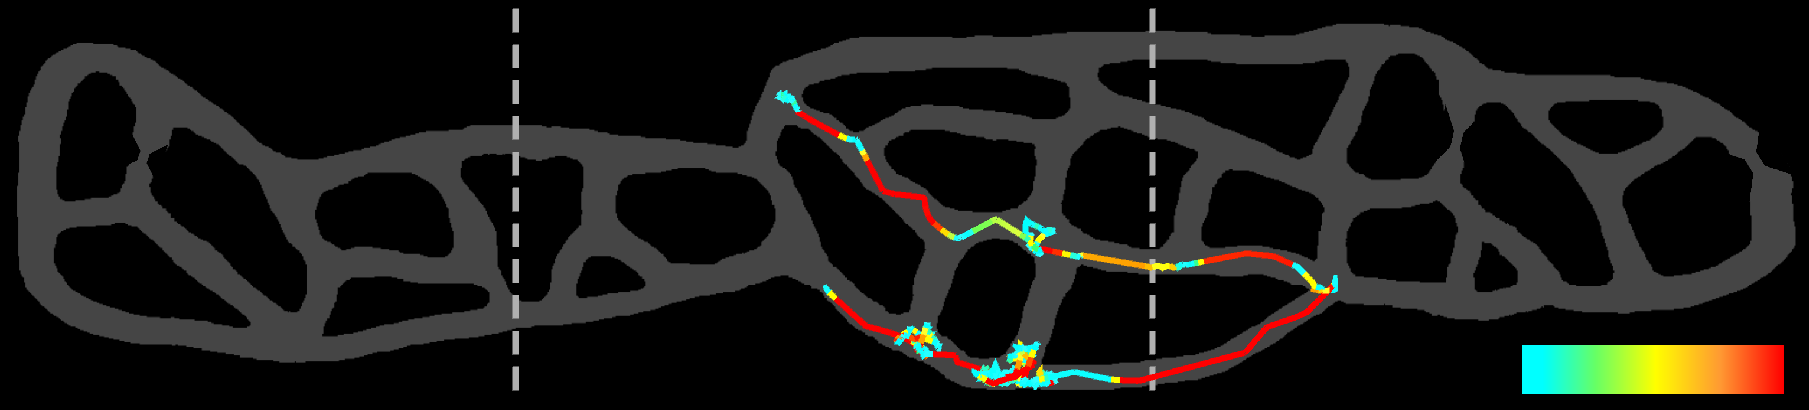
\includegraphics[width=\textwidth]{er-simulation-magic-particle}
	\caption[ER simulation: The simulated model shows similar particle velocity tracks to experimental data]{A single particle was tracked in the simulation, and its velocity recorded using the same colour scale as Figure~\ref{fig:ER-directed-flow-velocity}, where red shows fast particle velocity and blue slow velocity. The simulated model is in good agreement with experimental data, with fast directed movement along tubules and slower Brownian motion at junctions. Colour bar from slow (blue) to fast (red). }
	\label{fig:ER-simulation-magic-particle}
\end{figure}

To prevent too much energy being added to the network from multiple pinching events, collisions were inelastic and drag was added at network junctions to slow the particles.
Parameters were tuned to ensure the same average particle speed in the two mixing scenarios for a fair comparison.
A plot of a single particle's trajectory through the network is shown in Figure~\ref{fig:ER-simulation-magic-particle}, which is consistent with the experimental data in Figure~\ref{fig:er-directed-flow-velocity}, showing fast directed movement along tubules and slower Brownian motion at junctions.

Understanding the reason for ER pinching allows us to associate diseases with ER malfunction.
In cells with long projections, such as motor neurons, transporting luminal protein to remote parts of the cell quickly could be vital for healthy cellular function.

\section{Conclusion}
In~\cite{holcman2018single}, we present evidence that the movement of proteins in the ER is not diffusive, but also has an ATP-dependent directed-flow component.
By utilising the fast high-resolution imaging capabilities of LAG SIM, as well as computational simulation and analysis, this chapter has suggested that contraction of ER tubules is responsible for luminal flow.

Imaging at \SI{11}{\hertz} with \SI{80}{\nano\metre} resolution revealed ER networks in a dynamic equilibrium, constantly growing, shrinking, and rearranging.
Network analysis and tracking showed that this is not responsible for flow, however.

The capacity of ER to undergo reversible contractions was revealed when high laser power was used to image ER labelled with TMR, which caused blebbing in the network.
Rapid tubule pinching was revealed when re-examining individual segments of ER captured in TIRF-SIM mode.
The size and speed of the pinching phenomenon means that high-speed TIRF-SIM is currently the only technique able to visualise these events.

Using the Nvidia PhysX engine to perform simulations of proteins moving in the ER provided insight into the advantages of active flow over diffusion.
Tuning the simulation to maintain the same average particle speed in both the pinching and Brownian motion schemes, ensuring a fair comparison, showed that mixing occurs up to 3$\times$ faster in a network with pinching.
Pinching therefore reduces the time taken for proteins to reach remote areas of the network, such as by the cell membrane.
The interactive simulation is provided online at \url{https://laseranalyticsgroup.github.io/er}, where model parameters such as pinch size, particle size, and mean free path can be adjusted, for example to input values measured from electron microscopy data. 

Since ER is found in most eukaryotic cells, it is unsurprising that its malfunction is associated with a wide range of diseases.
By contributing to the community's fundamental understanding of ER mechanisms, we advance our capability for finding cures.

\section{Future research} \label{sec:ERfuture}
The dynamic rearrangement of the ER network has been observed by several groups~\cite{nixon2016increased, pendin2011balancing, yamanaka2018er}.
Furthermore is it now known that ER exhibits strong contact with all other organelles~\cite{valm2017applying, guo2018visualizing}.
Nevertheless, the biochemical mechanisms for network rearrangement are not well understood.

By utilising high-speed multi-colour SIM we have observed lysosomes localised at the endpoints of growing ER tubules, which appear to pull the network into its new shape.
Preliminary data, shown in Figure~\ref{fig:er-future}, indicates that ER tubules grow faster when assisted by lysosomes, and are also more likely to form new junctions by connecting to another area of the network than ER tubules growing without lysosomes.
Further investigation into specific proteins involved in this phenomenon are ongoing, as well as calculations into the dynamic forces required for ER network rearrangement.

\begin{figure}[htbp!]
	\centering
		\begin{subfigure}[b]{0.325\textwidth}
		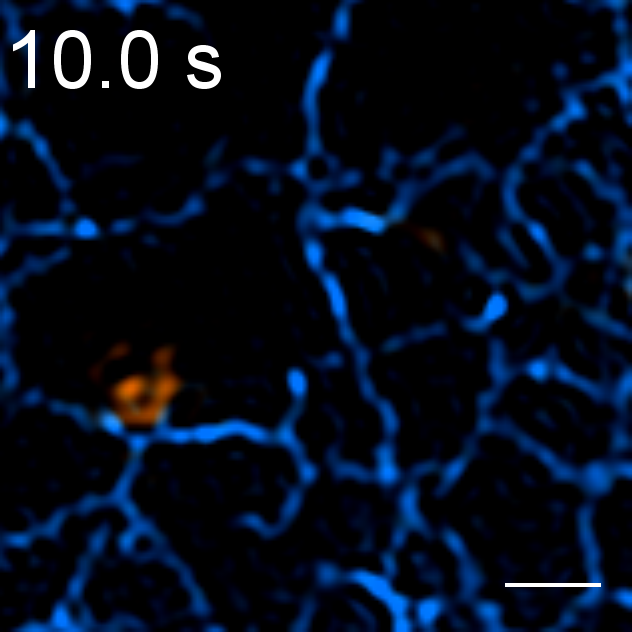
\includegraphics[width=1.0\textwidth]{er-future-1}
		\caption{} \label{fig:er-future-1}
	\end{subfigure}
	\hfill
	\begin{subfigure}[b]{0.325\textwidth}
		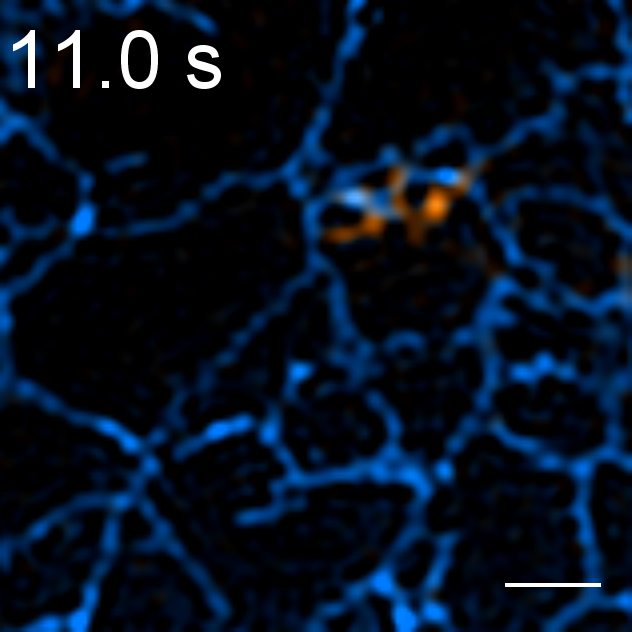
\includegraphics[width=1.0\textwidth]{er-future-2}
		\caption{} \label{fig:er-future-2}
	\end{subfigure}
	\hfill
	\begin{subfigure}[b]{0.325\textwidth}
		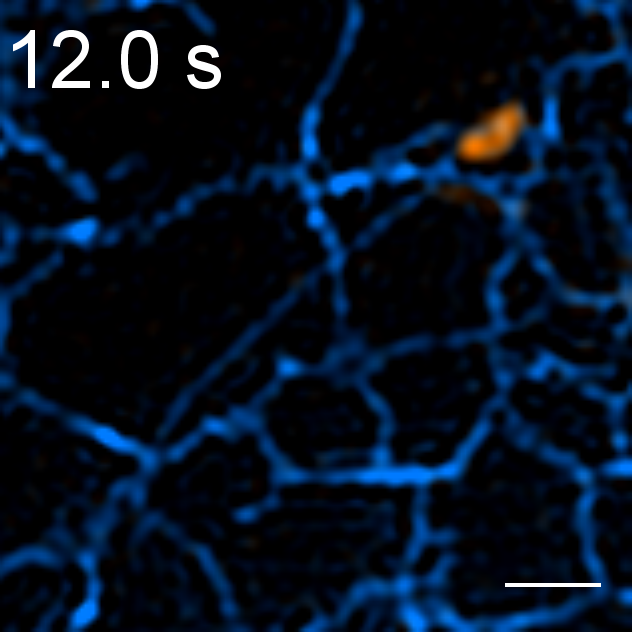
\includegraphics[width=1.0\textwidth]{er-future-3}
		\caption{} \label{fig:er-future-3}
	\end{subfigure}
	\caption[ER: Lysosomes form strong contacts with ER tubule endpoints to rearrange the network]{Preliminary multi-colour SIM data captured with the Optosplit shows lysosomes, coloured in orange, forming strong contacts with ER tubule endpoints, suggesting that lysosomes assist with rearrangement of the ER network. Scalebars are \SI{1}{\micro\metre}.}
	\label{fig:er-future}
\end{figure}
